\chapter{Roll center approximation}
\label{chap:roll}

The SAE definition of roll center is

\textit{\say{The point in the transverse vertical plane through any pair of wheel centers at which lateral forces may be applied to the sprung mass without producing suspension roll}}

This definition directly relates the $P_w$ points to the roll center height.
Validity for chosen roll center approximation can be shown by modifying a generic equilibrium situation such as the one described in figure \ref{roll} and applying a new side force $F'$ acting on the midpoint $M_F$ of $P_{FR}$ and $P_{FL}$, if the tyres are capable of generating the necessary friction forces ($F_1$ and $F_2$), the system will settle in a new equilibrium state.
The new situation is shown in figures \ref{rollforces} and A.2.

\begin{figure}[hbt]
  \centering
  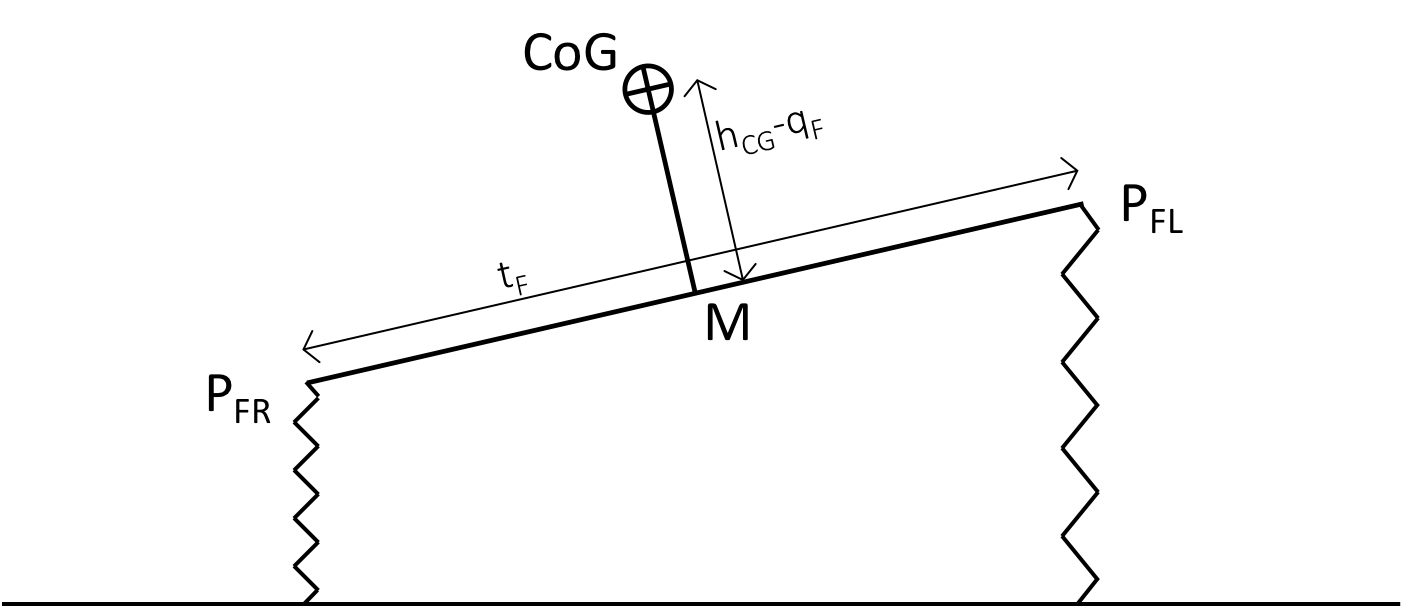
\includegraphics[height = 5cm]{images/rollsizes}
  \label{rollsizes}
  \caption{Front view of the front axle, dimensional parameters of the model.}

  \centering
  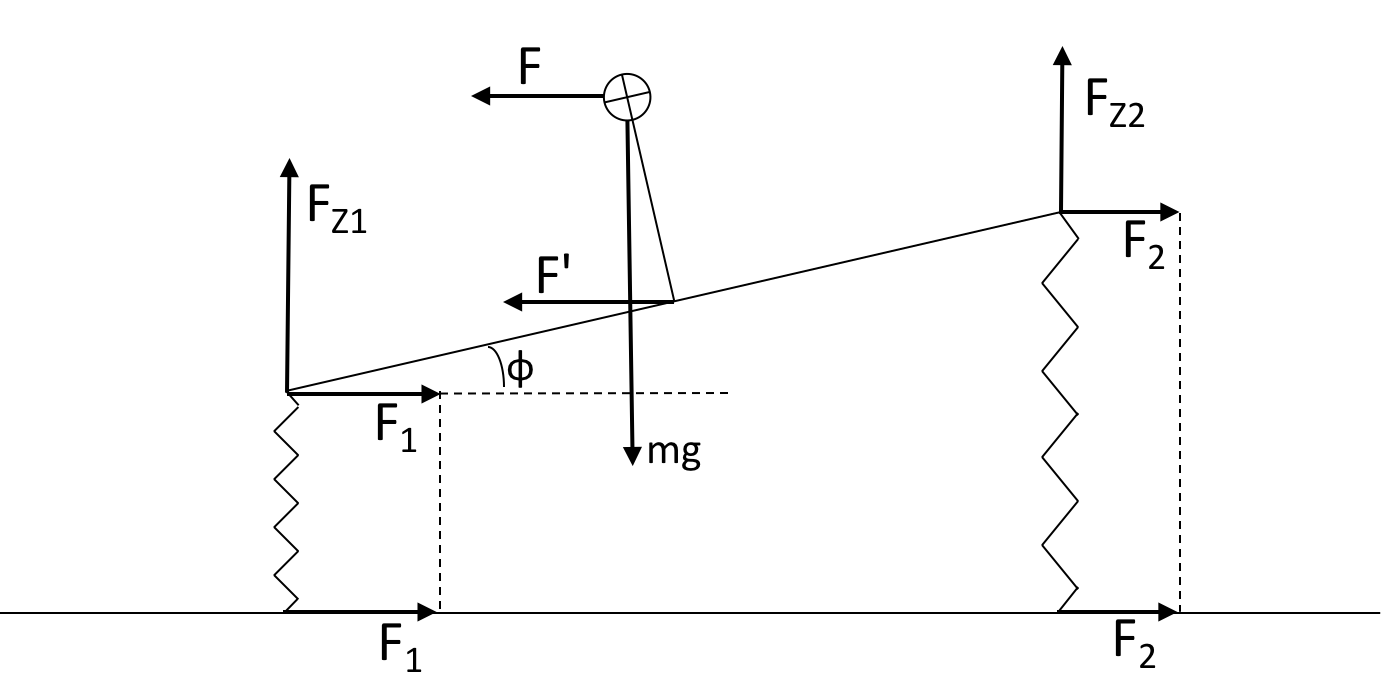
\includegraphics[height = 5cm]{images/rollforces}
  \label{rollforces}
  \caption{Front view of the front axle, forces acting on the vehicle.}

\end{figure}

The sum of vertical forces acting on the tyres does not change as it is equal to
$$
F_z := F_{z1}+F_{z2} = mg.
$$

As $F_z$ does not change, the increase in side friction force is entirely due to changes in the lateral friction coefficients, which are both supposed as being equal to $\mu_y$.

The fact that the spring systems are constrained in the vertical orientation means the horizontal forces acting at the ground contact points effect the chassis directly at the points $P_{FR}$ and $P_{FL}$ respectively.

The horizontal force balance is given by
$$
F + F' = F_1 + F_2 = \mu_y ( F_{z1} + F_{z2} ) = \mu_y mg
$$

To find the equilibrium roll angle the torque balance about point $M_F$ must be solved
$$
\frac{t_F}{2} \sin \phi (F_1-F_2) - \frac{t_F}{2} \cos \phi ( F_{z1} - F_{z2} ) - F (h_{CG}-q_F)  \cos \phi = 0
$$

substituting the friction forces yields
$$
\frac{t_F}{2} ( F_{z1} - F_{z2} ) [\mu_y \sin \phi - \cos \phi ] - F (h_{CG}-q_F)  \cos \phi = 0
$$

The vertical forces act through the springs (spring rate $k_F$) . As Hooke's law is linear, the difference between them is proportional to the difference between the spring lengths which is in turn obtained as a function of the roll angle.
$$
F_{z1} - F_{z2} = - k_F t_F \sin \phi
$$

The moment balance then becomes
$$
\mu_y k_F \frac{t_F^2}{2} \sin^2 \phi - k_F \frac{t_F^2}{2} \sin \phi \cos \phi - F(h_{CG}-q_F) \cos \phi = 0
$$

The roll angle in road vehicles rarely exceeds a few degrees so the equation may be linearized with respect to $\phi$.
$$
- k_F \frac{t_F^2}{2}  \phi  - F(h_{CG}-q_F) = 0
$$

Doing so makes the solution for $\phi$ independent of $\mu_y$, the only quantity influenced by $F'$. The height of point $M_F$ is then effectively the roll center height according to the SAE definition.

The roll rate $K_\phi$ is defined as roll angle per unit of lateral force applied to the CG, applying this definition to the linearized equation gives the expression to be used to derive spring rates for the 6DoF model in order to match the roll-rate of the car.
$$
K_\phi = \frac{\phi}{F} = 2\frac{h_{CG}-q_F}{K_Ft_F^2}
$$
